\chapter{Perancangan}
\label{chap:Perancangan}

Pada bab ini dibahas mengenai perancangan perangkat lunak yang dibangun, meliputi perancangan kelas dan algoritma pengecekan dokumen skripsi.

\section{Perancangan Kelas}
Pada bagian ini akan dijelaskan rancangan kelas yang akan digunakan pada perangkat lunak. Rancangan kelas tersebut akan ditunjukan oleh diagram kelas di bawah ini:

\begin{figure}[H]
	\centering	
	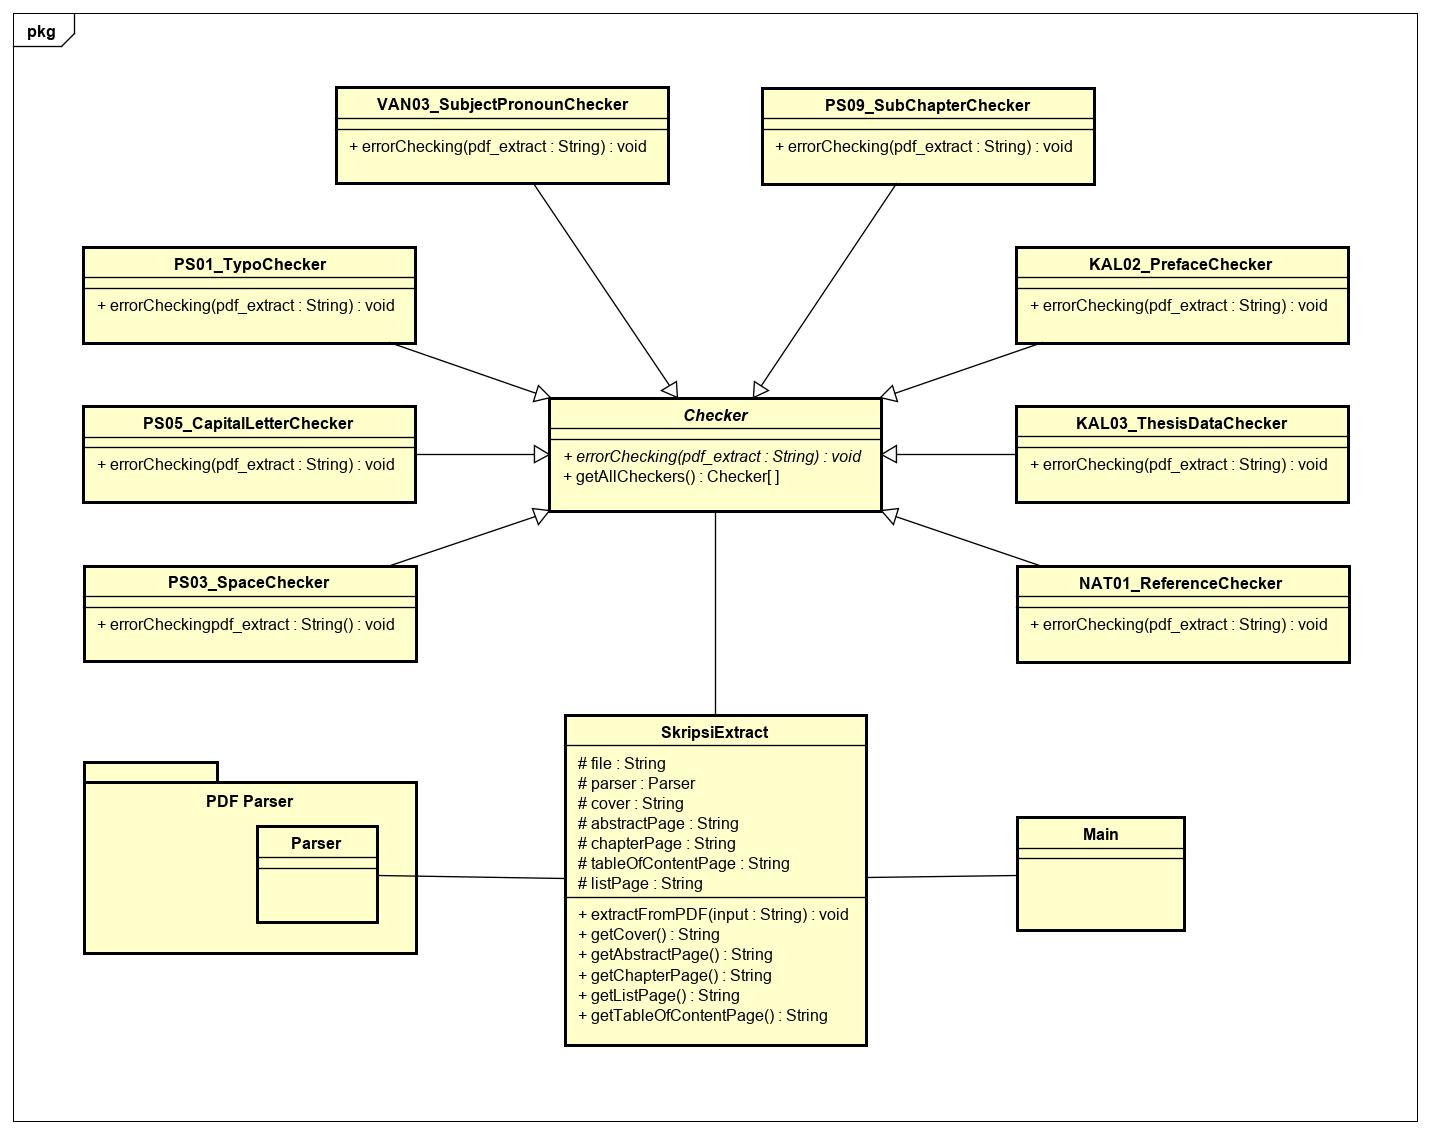
\includegraphics[scale=0.43]{class-diagram.png}
	\caption{Diagram kelas Aplikasi Pemeriksa Kesalahan Dokumen Skripsi}	
	\label{fig:diagram_kelas} 
\end{figure}

Pada gambar \ref{fig:diagram_kelas} telah ditunjukan bahwa perangkat lunak memiliki sebelas kelas. Rincian dari setiap kelas tersebut akan dijelaskan sebagai berikut:

\begin{enumerate}

	\item Kelas Checker \\
	Kelas ini merupakan kelas \textit{Parent} dari semua \textit{checker} yang menjadi fitur dari perangkat lunak. Berikut adalah \textit{method} yang terdapat pada kelas ini:
	
		\begin{itemize}
			\item errorChecking(\$pdf\_extract) \\
			Method ini merupakan method abstrak, yang akan diturunkan kepada seluruh anak kelasnya. Method ini berfungsi untuk memeriksa kesalahan pada dokumen skripsi sesuai dengan peran yang diberikan pada kelas tersebut. Method ini menerima masukan berupa array String pdf\_extract. Namun tidak semua isi dari array tersebut digunakan, bergantung dengan yang dibutuhkan oleh setiap kelas pemeriksa.			
			
			\item getAllChecker() \\
			Method ini berfungsi untuk melakukan instansiasi seluruh anak kelas \textit{Checker}. Method ini mengembalikan hasil instansiasi anak kelas \textit{Checker}.
		\end{itemize}
	
	\item Kelas KAL02\_PrefaceChecker \\
	Kelas ini digunakan untuk memeriksa kata pengantar pada setiap bab dan subbab. Berikut adalah \textit{method} yang terdapat pada kelas ini:
	
		\begin{itemize}
			\item errorChecking(\$pdf\_extract) \\
			Method ini berfungsi untuk memeriksa kesalahan pada dokumen skripsi. Method ini menerima masukan berupa array String pdf\_extract. Bagian yang diperiksa pada kelas ini hanya bab 1 hingga bab 6.
		\end{itemize}
	
	\item Kelas KAL03\_ThesisDataChecker \\
	Kelas ini digunakan untuk memeriksa kelengkapan data skripsi dalam bahasa Indonesia dan bahasa Inggris. Berikut adalah \textit{method} yang terdapat pada kelas ini:
			
		\begin{itemize}
			\item errorChecking(\$pdf\_extract) \\
			Method ini berfungsi untuk memeriksa kesalahan pada dokumen skripsi. Method ini menerima masukan berupa array String pdf\_extract.
		\end{itemize}
		
	\item Kelas NAT01\_ReferenceChecker \\
	Kelas ini digunakan untuk memeriksa referensi yang akan dirujuk dalam dokumen. Berikut adalah \textit{method} yang terdapat pada kelas ini:
	
		\begin{itemize}
			\item errorChecking(\$pdf\_extract) \\
			Method ini berfungsi untuk memeriksa kesalahan pada dokumen skripsi. Method ini menerima masukan berupa array String pdf\_extract.
		\end{itemize}
			
	\item Kelas PS01\_TypoChecker \\
	Kelas ini digunakan untuk memeriksa kesalahan penulisan kata. Berikut adalah \textit{method} yang terdapat pada kelas ini:
	
		\begin{itemize}
			\item errorChecking(\$pdf\_extract) \\
			Method ini berfungsi untuk memeriksa kesalahan pada dokumen skripsi. Method ini menerima masukan berupa array String pdf\_extract.
		\end{itemize}
			
	\item Kelas PS03\_SpaceChecker \\
	Kelas ini digunakan untuk memeriksa penggunaan spasi sebelum dan setelah tanda baca. Berikut adalah \textit{method} yang terdapat pada kelas ini:	
	
		\begin{itemize}
			\item errorChecking(\$pdf\_extract) \\
			Method ini berfungsi untuk memeriksa kesalahan pada dokumen skripsi. Method ini menerima masukan berupa array String pdf\_extract.
		\end{itemize}
			
	\item Kelas PS05\_CapitalLetterChecker \\
	Kelas ini digunakan untuk memeriksa penggunaan huruf kapital pada awal kalimat. Berikut adalah \textit{method} yang terdapat pada kelas ini:
		
		\begin{itemize}
			\item errorChecking(\$pdf\_extract) \\
			Method ini berfungsi untuk memeriksa kesalahan pada dokumen skripsi. Method ini menerima masukan berupa array String pdf\_extract.
		\end{itemize}
			
	\item Kelas PS09\_SubChapterChecker \\
	Kelas ini digunakan untuk memeriksa subbab yang ada dalam sebuah bab. Berikut adalah \textit{method} yang terdapat pada kelas ini:
			
		\begin{itemize}
			\item errorChecking(\$pdf\_extract) \\
			Method ini berfungsi untuk memeriksa kesalahan pada dokumen skripsi. Method ini menerima masukan berupa array String pdf\_extract.
		\end{itemize}
			
	\item Kelas VAN03\_SubjectProunounChecker \\
	Kelas ini digunakan untuk memeriksa penggunaan kata ganti orang pada dokumen skripsi. Berikut adalah \textit{method} yang terdapat pada kelas ini:
	
		\begin{itemize}
			\item errorChecking(\$pdf\_extract) \\
			Method ini berfungsi untuk memeriksa kesalahan pada dokumen skripsi. Method ini menerima masukan berupa array String pdf\_extract.
		\end{itemize}
			
	\item Kelas SkripsiExtract \\
	kelas ini digunakan untuk melakukan ekstaksi file PDF skripi. Berikut adalah \textit{method} yang terdapat pada kelas ini:
	
	\item Kelas Main \\
	Kelas ini digunakan untuk menjalankan perangkat lunak.

\end{enumerate} 

\section{Algoritma Pengecekan}
Pada bagian ini akan dijelaskan algoritma pengecekan yang akan digunakan pada perangkat lunak. Hasil survei kesalahan-kesalahan dalam penulisan dokumen skripsi sudah disaring dan akan diimplementasikan dalam perangkat lunak. Pengecekan kesalahan tersebut akan dilakukan dengan menggunakan teknik \textit{pattern matching regex}. Berikut adalah rincian dari hasil survei yang dipilih beserta penyelesaiannya:

\begin{enumerate}
	\item Penulisan kata (PS-01) \\
	Untuk mendeteksi kesalahan penulisan kata, akan digunakan ekstensi kamus bahasa Indo10
nesia \textit{LibreOffice}. Dengan digunakan kamus tersebut, kesalahan penulisan suatu kata dapat diminimalisir. \newline
	Penyelesaian dengan \textit{regex}:
	
	\item Pemberian spasi sebelum dan sesudah tanda baca (PS-03) \\
	Kesalahan ini akan terdeteksi apabila tidak ada karakter spasi sebelum ataupun sesudah tanda baca.
	Penyelesaian dengan \textit{regex}:
	
	\item Awal kalimat tidak menggunakan huruf kapital (PS-05) \\
	Kesalahan ini akan terdeteksi apabila setelah tanda baca pada akhir kalimat, karakter pertama setelah spasi menggunakan huruf kecil.	
	Penyelesaian dengan \textit{regex}:
	
	\item Jumlah subbab dalam 1 bab tidak boleh hanya 1 (PS-09) \\
	Kesalahan ini dapat diselesaikan dengan mencari jumlah subbab yang ada dalam sebuah bab. \newline:
	Penyelesaian dengan \textit{regex}:
	
	\item Kalimat pengantar untuk setiap subbab (KAL-02) \\
	Kesalahan ini dapat dideteksi dengan melihat ada atau tidaknya kalimat setelah subbab dibuat. \newline
	Penyelesaian dengan \textit{regex}:
	
	\item Kelengkapan data skripsi (KAL-03) \\
	Kesalahan ini dapat terlihat pada halaman cover skripsi. Mahasiswa yang belum mengisi data skripsi, pada file PDFnya akan ditampilkan tulisan template pada data skripsinya. \newline
	Penyelesaian dengan \textit{regex}:
	
	\item Penggunaan kata ganti orang (VAN-03) \\
	Kesalahan ini dapat diatasi dengan memasukan kata-kata yang termasuk dalam kata ganti orang menjadi kata-kata yang tidak dapat digunakan. \newline
	Penyelesaian dengan \textit{regex}:
	
	\item Penulisan daftar referensi (NAT-01) \\
	Kesalahan dalam penulisan daftar referensi dapat dilihat dengan munculnya tanda ''[?]''. \newline
	Penyelesaian dengan \textit{regex}:
	
\end{enumerate}